\documentclass[11pt]{beamer}

% Theme and packages
\usetheme{Madrid}
\usecolortheme{default}
\useoutertheme{default} % removes bottom bars
\setbeamertemplate{footline}{} % removes footer bar
\setbeamertemplate{navigation symbols}{} % removes navigation icons

\usepackage{amsmath, amssymb, amsfonts}
\usepackage{tikz}
\usetikzlibrary{shapes.geometric, arrows}
\usepackage{fancyvrb}

% Flowchart styles
\tikzstyle{startstop} = [rectangle, rounded corners, minimum width=3cm, minimum height=1cm,text centered, draw=black, fill=red!30]
\tikzstyle{process} = [rectangle, minimum width=3cm, minimum height=1cm, text centered, draw=black, fill=blue!20]
\tikzstyle{decision} = [diamond, aspect=2, text centered, minimum width=3cm, draw=black, fill=green!20]
\tikzstyle{arrow} = [thick,->,>=stealth]

% Title information
\title[Factorization of Ideals]{Factorization of Algebraic Ideals and Its Applications}
\author{Brent Baccala}
\institute{freesoft.org}
\date{October 1, 2025}

\begin{document}

%----------------------------------
% Title Slide
%----------------------------------
\begin{frame}
  \titlepage
\end{frame}

%----------------------------------
\begin{frame}{Motivation}
\begin{itemize}
  \item Ideal decomposition simplifies systems of polynomial equations.
  \item Provides structure for algebraic and geometric analysis.
  \item Fundamental tool for both theory and computation.
\end{itemize}
\end{frame}

%----------------------------------
\begin{frame}{Background: Ideals in Commutative Algebra}
\begin{columns}
\column{0.55\textwidth}
\begin{itemize}
  \item An \textbf{ideal} $I \subset R$ is a subset closed under addition and multiplication by ring elements.
  \item \textbf{Prime ideal:} if $ab \in P$, then $a \in P$ or $b \in P$.
  \item \textbf{Primary ideal:} if $ab \in Q$, then $a \in Q$ or $b^n \in Q$.
\end{itemize}
\column{0.45\textwidth}
\centering
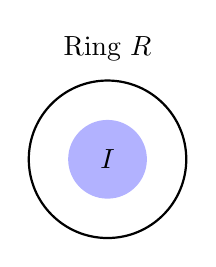
\begin{tikzpicture}
  \draw[thick] (0,0) circle (1);
  \node at (0,1.4) {Ring $R$};
  \fill[blue!30] (0,0) circle (0.5);
  \node at (0,0) {$I$};
\end{tikzpicture}
\end{columns}
\end{frame}

%----------------------------------
\begin{frame}{Prime and Primary Decomposition}
\begin{columns}
\column{0.55\textwidth}
\begin{itemize}
  \item Decomposing an ideal as an intersection of prime ideals.
  \item Geometric viewpoint: corresponds to union of algebraic varieties.
  \item Analogy with integer factorization.
\end{itemize}
\column{0.45\textwidth}
\centering
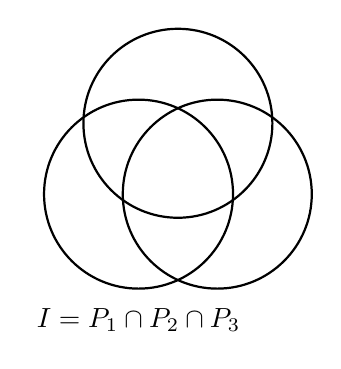
\begin{tikzpicture}
  \draw[thick] (0,0) circle (1.2);
  \draw[thick] (1,0) circle (1.2);
  \draw[thick] (0.5,0.9) circle (1.2);
  \node at (0, -1.6) {$I = P_1 \cap P_2 \cap P_3$};
\end{tikzpicture}
\end{columns}
\end{frame}

%----------------------------------
\begin{frame}{Classical Results}
\begin{itemize}
  \item \textbf{Lasker–Noether theorem}: Every ideal in a Noetherian ring admits a primary decomposition.
  \item Uniqueness up to radicals and associated primes.
\end{itemize}
\end{frame}

%----------------------------------
\begin{frame}{Algorithms for Ideal Factorization}
\centering
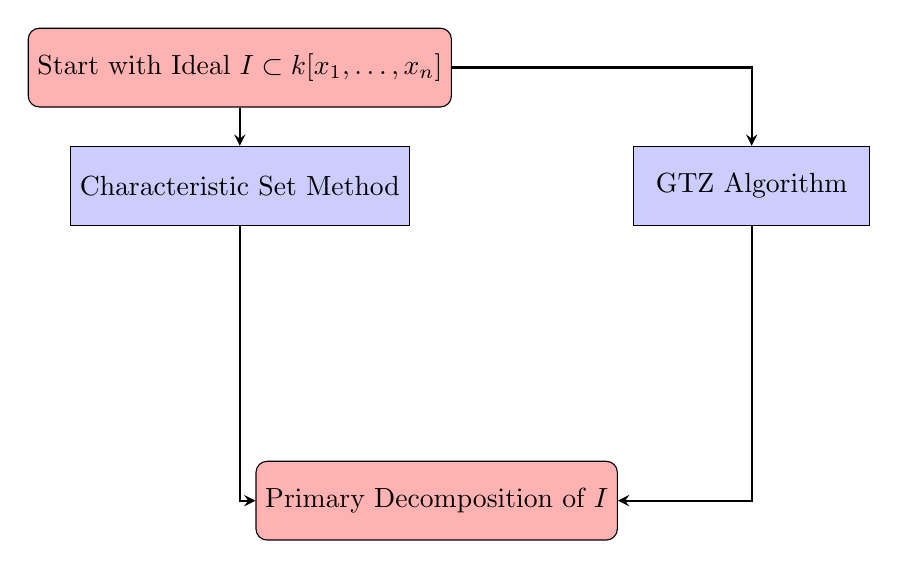
\begin{tikzpicture}[node distance=1.5cm]
\node (start) [startstop] {Start with Ideal $I \subset k[x_1,\dots,x_n]$};
\node (cs) [process, below of=start] {Characteristic Set Method};
\node (gtz) [process, right of=cs, xshift=5cm] {GTZ Algorithm};
\node (end) [startstop, below of=cs, yshift=-2.5cm, xshift=2.5cm] {Primary Decomposition of $I$};

\draw [arrow] (start) -- (cs);
\draw [arrow] (start) -| (gtz);
\draw [arrow] (cs) |- (end);
\draw [arrow] (gtz) |- (end);
\end{tikzpicture}
\end{frame}

%----------------------------------
\begin{frame}{Characteristic Set Method}
\begin{itemize}
  \item Uses elimination and triangular sets.
  \item Originates in differential algebra.
  \item Advantage: systematic structure.
  \item Limitation: ordering choice is crucial.
\end{itemize}
\end{frame}

%----------------------------------
\begin{frame}{GTZ Algorithm}
\begin{itemize}
  \item Gröbner basis-based.
  \item Splits and refines components iteratively.
  \item Widely implemented in CAS.
\end{itemize}
\centering
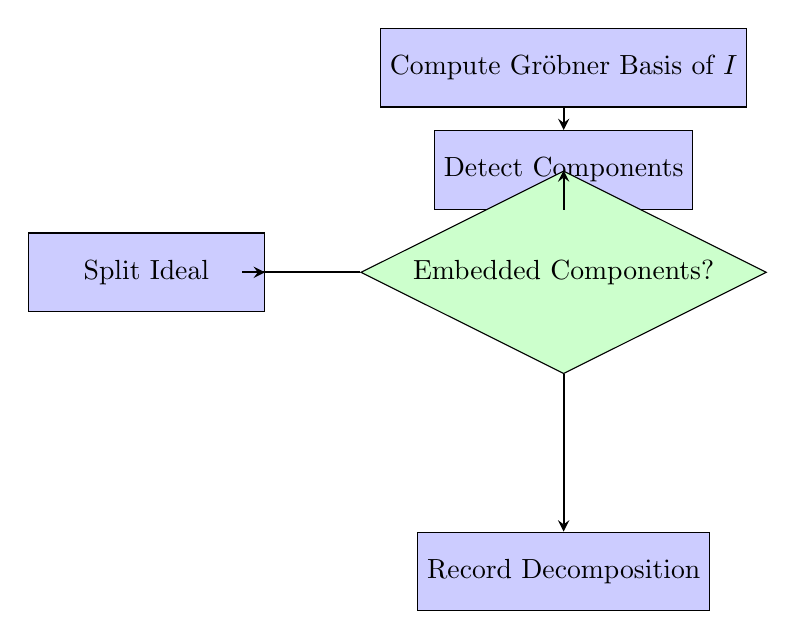
\begin{tikzpicture}[node distance=1.3cm]
\node (gb) [process] {Compute Gröbner Basis of $I$};
\node (comp) [process, below of=gb] {Detect Components};
\node (split) [decision, below of=comp] {Embedded Components?};
\node (splityes) [process, left of=split, xshift=-4cm] {Split Ideal};
\node (no) [process, below of=split, yshift=-2.5cm] {Record Decomposition};

\draw [arrow] (gb) -- (comp);
\draw [arrow] (comp) -- (split);
\draw [arrow] (split.west) -- ++(-1.5,0) -- (splityes.east);
\draw [arrow] (split.south) -- ++(0,-1) -- (no.north);
\end{tikzpicture}
\end{frame}

%----------------------------------
\begin{frame}{Worked Example 1}
\begin{itemize}
  \item Example: $I = \langle x^2-y, \, xy \rangle \subset k[x,y]$
  \item Gröbner basis computation $\rightarrow$ decomposition.
  \item Interpreted geometrically as simpler varieties.
\end{itemize}
\centering
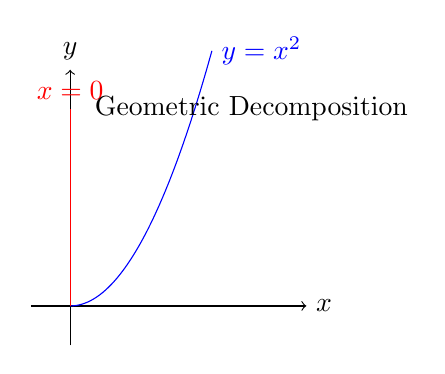
\begin{tikzpicture}
  \draw[->] (-0.5,0) -- (3,0) node[right] {$x$};
  \draw[->] (0,-0.5) -- (0,3) node[above] {$y$};
  \draw[domain=0:1.8,smooth,variable=\x,blue] plot ({\x},{\x*\x}) node[right] {$y=x^2$};
  \draw[red] (0,0) -- (0,2.5) node[above] {$x=0$};
  \node at (2.3,2.5) {Geometric Decomposition};
\end{tikzpicture}
\end{frame}

%----------------------------------
\begin{frame}{Applications to Polynomial Equations}
\begin{itemize}
  \item Decomposition $\Leftrightarrow$ splitting solution sets.
  \item Ideal $\cap$ decomposition $\Rightarrow$ variety union.
\end{itemize}
\centering
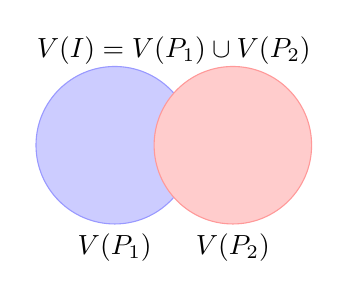
\begin{tikzpicture}
  \draw[blue!40,fill=blue!20] (0,0) circle(1);
  \draw[red!40,fill=red!20] (1.5,0) circle(1);
  \node at (0,-1.3) {$V(P_1)$};
  \node at (1.5,-1.3) {$V(P_2)$};
  \node at (0.75,1.2) {$V(I)=V(P_1)\cup V(P_2)$};
\end{tikzpicture}
\end{frame}

%----------------------------------
\begin{frame}{Applications to Differential Equations}
\begin{itemize}
  \item Characteristic set methods connect differential systems with ideals.
  \item Decomposition splits families of solutions.
\end{itemize}
\end{frame}

%----------------------------------
\begin{frame}{Current Limits and Open Problems}
\begin{itemize}
  \item Complexity is often exponential.
  \item Gröbner basis can be costly.
  \item Future directions:
    \begin{itemize}
      \item Hybrid and numerical-symbolic methods.
      \item Parallelization.
    \end{itemize}
\end{itemize}
\end{frame}

%----------------------------------
\begin{frame}[fragile]{Profiling Singular (data collection)}

A large polynomial system (33 variables, 3486 equations, 16,517,523 terms) over $\mathbb{F}_{536870909}$ is in {\tt helium-16.6-R536870909}

\vskip 12pt

In one window, we run the calculation:

{\tiny\begin{verbatim}
baccala@samsung:~/src/helium$ ../sage/sage
sage: import pickle
sage: with open('helium-16.6-R536870909', 'rb') as f:
....:     eqns = pickle.load(f)
....: 
sage: I = ideal(eqns)
sage: bwb = I.minimal_associated_primes()
\end{verbatim}}

In another window, we profile it:

{\tiny\begin{verbatim}
baccala@samsung:~/src/helium$ ps ax | grep sage
 148747 pts/4    S+     0:00 /bin/sh /home/baccala/src/sage/src/bin/sage-python /home/baccala/src/sage/src/bin/sage-ipython -i
 148818 pts/4    S+     0:00 /bin/sh /home/baccala/src/sage/src/bin/sage-python /home/baccala/src/sage/src/bin/sage-cleaner
 148819 pts/4    S+     0:00 python3 /home/baccala/src/sage/src/bin/sage-cleaner
 148820 pts/4    Rl+    0:51 python3 /home/baccala/src/sage/src/bin/sage-ipython -i
 148985 pts/1    S+     0:00 grep --color=auto sage
baccala@samsung:~/src/helium$ perf record --call-graph dwarf -g -p 148820 sleep 30
\end{verbatim}}
\end{frame}


%----------------------------------
\begin{frame}[fragile]{Profiling Singular (data analysis)}
\tiny\begin{verbatim}
baccala@samsung:~/src/helium$ perf report

    99.86%     0.00%  python3  libSingular-4.4.1.so                      [.] yyparse()
            |
            ---yyparse()
               iiExprArithM(sleftv*, sleftv*, int)
               iiExprArith1Tab(sleftv*, sleftv*, int, sValCmd1 const*, int, sConvertTypes const*)
               jjSTD(sleftv*, sleftv*)
               kStd_internal(sip_sideal*, sip_sideal*, tHomog, intvec**, bigintmat*, int, int, intvec*, int (*)(skStrategy*))
               bba(sip_sideal*, sip_sideal*, intvec*, bigintmat*, skStrategy*)
               |          
                --99.34%--enterpairs(spolyrec*, int, int, int, skStrategy*, int)
                          |          
                           --99.34%--initenterpairs(spolyrec*, int, int, int, skStrategy*, int)
                                     |          
                                     |--84.24%--chainCritNormal(spolyrec*, int, skStrategy*)
                                     |          |          
                                     |          |--81.56%--kMergeBintoL(skStrategy*)
                                     |          |          |          
                                     |          |           --81.40%--__memcpy_avx_unaligned_erms (inlined)
                                     |          |          
                                     |           --2.68%--deleteIfCompareChain(spolyrec*, int, skStrategy*, int (*)(spolyrec*, spolyrec*, spolyrec*, spolyrec*, ip_sring*), bool, bool, bool)
                                     |                     |          
                                     |                      --2.60%--pCompareChain(spolyrec*, spolyrec*, spolyrec*, spolyrec*, ip_sring*)
                                     |          
                                     |--13.77%--deleteIfAble(spolyrec*, skStrategy*, bool)
                                     |          |          
                                     |           --4.17%--isPairsetInL(std::reverse_iterator<__gnu_cxx::__normal_iterator<sLObject*, std::vector<sLObject, std::allocator<sLObject> > > >&, spolyrec*, spolyrec*, skStrategy*)
                                     |          
                                      --1.32%--enterOnePairNormal(int, spolyrec*, int, int, skStrategy*, int)
\end{verbatim}
\end{frame}


%----------------------------------
\begin{frame}[fragile]{A Buggy Comparator}
\tiny\begin{verbatim}
int posInL110 (const LSet set, const int length, LObject* p,const kStrategy) {
  if (length<0) return 0;

  int o = p->GetpFDeg();
  int op = set[length].GetpFDeg();
  int cmp_int= -currRing->OrdSgn;

  if ((op > o)
  || ((op == o) && (set[length].length >p->length))
  || ((op == o) && (set[length].length <= p->length) && (pLmCmp(set[length].p,p->p) != cmp_int)))
    return length+1;
  int i;
  int an = 0;
  int en= length;
  loop
  {
    if (an >= en-1)
    {
      op = set[an].GetpFDeg();
      if ((op > o)
      || ((op == o) && (set[an].length >p->length))
      || ((op == o) && (set[an].length <=p->length) && (pLmCmp(set[an].p,p->p) != cmp_int)))
        return en;
      return an;
    }
    i=(an+en) / 2;
    op = set[i].GetpFDeg();
    if ((op > o)
    || ((op == o) && (set[i].length > p->length))
    || ((op == o) && (set[i].length <= p->length) && (pLmCmp(set[i].p,p->p) != cmp_int)))
      an=i;
    else
      en=i;
  }
}
\end{verbatim}
\end{frame}

%----------------------------------
\begin{frame}{The Big Picture}
\small
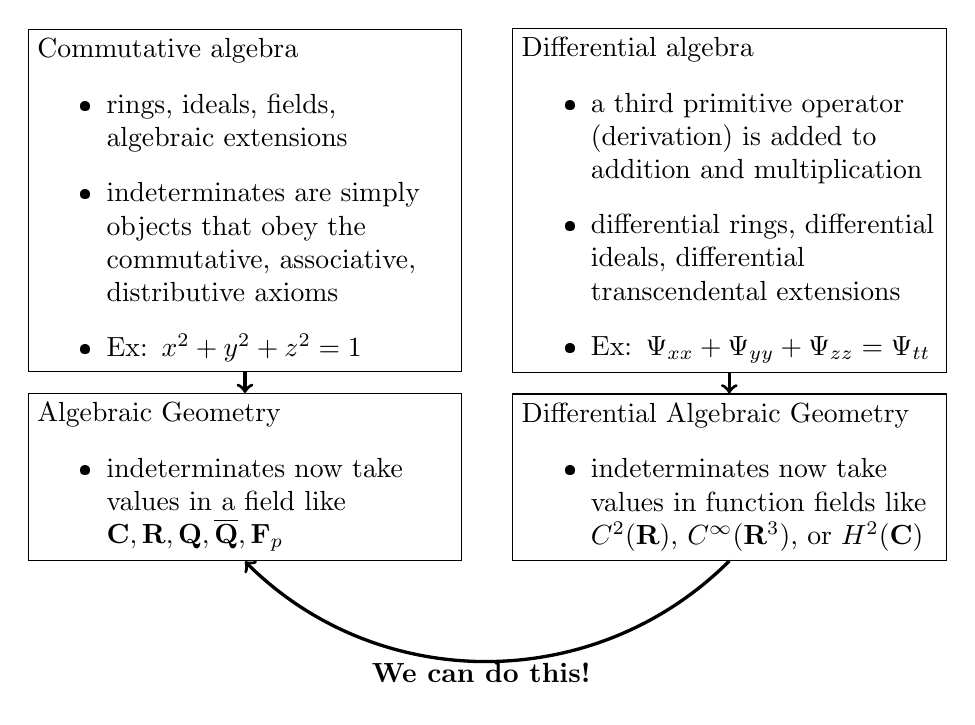
\begin{tikzpicture}[node distance=20pt]
\node (commutative algebra) [draw, text width=150pt] {Commutative algebra
      \begin{itemize}
        \item rings, ideals, fields, algebraic extensions
        \item indeterminates are simply objects that obey the commutative, associative, distributive axioms
        \item Ex: $x^2+y^2+z^2=1$
      \end{itemize}
};
\node (algebraic geometry) [draw, node distance=100pt, below of=commutative algebra, text width=150pt] {Algebraic Geometry
      \begin{itemize}
        \item indeterminates now take values in a field like $\mathbf{C}, \mathbf{R}, \mathbf{Q}, \overline{\mathbf{Q}}, \mathbf{F}_p$
      \end{itemize}
};
\node (differential algebra) [draw, node distance=175pt, right of=commutative algebra, text width=150pt] {Differential algebra
      \begin{itemize}
        \item a third primitive operator (derivation) is added to addition and multiplication
        \item differential rings, differential ideals, differential transcendental extensions
        \item Ex: $\Psi_{xx}+\Psi_{yy}+\Psi_{zz}=\Psi_{tt}$
      \end{itemize}
};
\node (differential algebraic geometry) [draw, node distance=100pt, below of=differential algebra, text width=150pt] {Differential Algebraic Geometry
      \begin{itemize}
        \item indeterminates now take values in function fields like $C^2(\mathbf{R})$,
$C^\infty(\mathbf{R}^3)$, or $H^2(\mathbf{C})$
      \end{itemize}
};

\draw [very thick, ->] (commutative algebra.south) -- (algebraic geometry.north);
\draw [very thick, ->] (differential algebra.south) -- (differential algebraic geometry.north);

\draw [very thick, ->] (differential algebraic geometry.south) to[out=-135, in=-45] (algebraic geometry.south);

\node at (3,-6) {\bf We can do this!};

\end{tikzpicture}
\end{frame}

%----------------------------------
\begin{frame}{Summary and Conclusions}
\begin{itemize}
  \item Every ideal in a Noetherian ring can be decomposed.
  \item Algorithms (Characteristic Set, GTZ) make this practical.
  \item Applications: polynomial and differential systems.
\end{itemize}
\end{frame}

%----------------------------------
\begin{frame}{Questions?}
  \centering
  \Huge Thank you! \\
  \vspace{1cm}
  \Large Questions welcome.
\end{frame}

\end{document}
